
\section{Statistical learning}
\subsection{Supervised learning}
\begin{frame}[t]{The goal of statistical learning}
\begin{center}
\tikzset{tbox/.style={draw, text badly centered, very thick, black, rectangle, inner sep=0, minimum width = 2.0 cm, minimum height = 1.0 cm}}
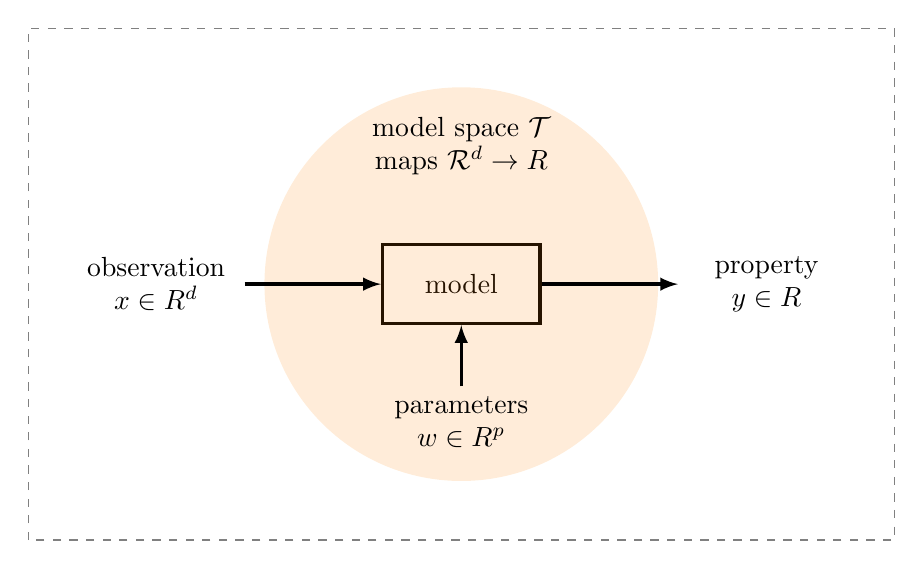
\begin{tikzpicture}[x=1cm,y=1cm, text badly centered]
%\pgfresetboundingbox
\draw[use as bounding box, anchor = north west,draw,dashed,gray] (-5.5,-3.25) rectangle (5.5,3.25);
\clip (-5.5,-3.25) rectangle (5.5,3.25);
\visible<2->{\node[anchor=west, text width=2 cm] (obs) at (-5.0,0) {observation $x\in\mathbb{R}^{d}$};}
\visible<5->{\node [tbox,minimum width=2.0 cm, text width = 2.0 cm] (model) at (0,0) {model};}
\visible<2->{\node[anchor=east, text width=2 cm] (preds) at (5.0,0) {property $y\in\mathbb{R}$};}
\visible<3->{\node[circle,minimum size=5cm, fill=orange, opacity=0.15,text opacity=1.0] at (0,0){};}
\visible<3->{\node[text width=2.5 cm, text badly centered]  at (0,1.75){model space $\mathcal{T}$ maps $\mathcal{R}^{d}\rightarrow \mathbb{R}$};}
\visible<4->{\node[text width=2.5 cm] (params) at (0,-1.75){parameters $w\in\mathbb{R}^{p}$};}
%% paths
\visible<5->{\path[draw,very thick,->] (obs) -- (model);}
\visible<5->{\path[draw,very thick,->] (model) -- (preds);}
\visible<5->{\path[draw,very thick,->] (params) -- (model);}
\end{tikzpicture}
\end{center}
\end{frame}
\begin{frame}[t]{Overview of supervised learning}
\begin{center}
\vspace{-0.5cm}
\tikzstyle{block} = [rectangle, draw, fill=blue!20,
text width=1.5cm, text centered, rounded corners, minimum height=1.5cm]	
\def\rectDiv#1#2#3#4#5{%#columns, #rows, rectangle start, rectangle end, list of elements to fill
\draw #3 rectangle #4;
\path #3;
\pgfgetlastxy{\firstx}{\firsty}
\path #4;
\pgfgetlastxy{\secondx}{\secondy}
\pgfmathsetlengthmacro{\xdiff}{\secondx-\firstx}
\pgfmathsetlengthmacro{\ydiff}{\secondy-\firsty}
\pgfmathsetlengthmacro{\myxstep}{\xdiff/#1}
\pgfmathsetlengthmacro{\myystep}{\ydiff/#2}
\foreach \x in {1,...,#1}{
	\draw ($#3 +\x*(\myxstep,0)$) -- ($#3 +(0,\ydiff) +\x*(\myxstep,0)$);
}
\foreach \y in {1,...,#2}{
	\draw ($#3 +\y*(0,\myystep)$) -- ($#3 +(\xdiff,0) +\y*(0,\myystep)$);
}
\foreach \i/\j in {#5}{
	\path[fill=darkgreen!20,draw] ($#3 + (\i*\myxstep,\j*\myystep)$) rectangle ($#3 + (\i*\myxstep,\j*\myystep) + (\myxstep,\myystep)$);
}
}
\def\rectDivred#1#2#3#4#5{%#columns, #rows, rectangle start, rectangle end, list of elements to fill
\draw #3 rectangle #4;
\path #3;
\pgfgetlastxy{\firstx}{\firsty}
\path #4;
\pgfgetlastxy{\secondx}{\secondy}
\pgfmathsetlengthmacro{\xdiff}{\secondx-\firstx}
\pgfmathsetlengthmacro{\ydiff}{\secondy-\firsty}
\pgfmathsetlengthmacro{\myxstep}{\xdiff/#1}
\pgfmathsetlengthmacro{\myystep}{\ydiff/#2}
\foreach \x in {1,...,#1}{
	\draw ($#3 +\x*(\myxstep,0)$) -- ($#3 +(0,\ydiff) +\x*(\myxstep,0)$);
}
\foreach \y in {1,...,#2}{
	\draw ($#3 +\y*(0,\myystep)$) -- ($#3 +(\xdiff,0) +\y*(0,\myystep)$);
}
\foreach \i/\j in {#5}{
	\path[fill=red!20,draw] ($#3 + (\i*\myxstep,\j*\myystep)$) rectangle ($#3 + (\i*\myxstep,\j*\myystep) + (\myxstep,\myystep)$);
}
}
\tikzset{tbox/.style={draw, text badly centered, very thick, black, rectangle, inner sep=0, minimum width = 2.0 cm, minimum height = 1.0 cm}}
\begin{tikzpicture}[x=1cm,y=1cm]
%\pgfresetboundingbox
\draw[use as bounding box, anchor = north west,draw,dashed,gray] (-2,-3.5) rectangle (9.5,3.5);
\clip (-2,-3.25) rectangle (9.0,3.25);
\node (ds) at (0,0){};
\node (dsy) at (0,4){};
\node (dsx) at (4,0){};
\def \cssize {1.0 cm}
\def \psize {1.15 cm}
\def\circledarrow#1#2#3{ % #1 Style, #2 Center, #3 Radius
	\draw[#1,->] (#2) +(80:#3) arc(80:-260:#3);}
%% now the flow chart
%% define coordinate grid 
\def \xfarleft {1}
\def \xleft {2.5}
\def \xmid {5.25}
\def \xright {8}
\def \ytop {2.75}
\def \ymid {0.5}
\def \ybot {-2.5}
\def \yphasetwo {-2.0}
\def \xlabeloffset {0.05}
\def \ylabeloffset {0.15}

%% title/step tracking
\node[anchor=north west] (title) at (4,3.3) {\large 
	\only<1>{\textbf{1. Collect data ($X,y$)}}
	\only<2>{\textbf{2. Featurize}}
	\only<3-4>{\textbf{3. Partition data}}
	\only<5-10>{\textbf{4. Learning phase}}
	\only<11->{\textbf{5. Testing phase}}
};


%% molecules
\only<1-2>{
{\node[circle,draw, thick, minimum width =\cssize,path picture={\node at (path picture bounding box.center){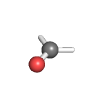
\includegraphics[width= \psize]{satistical_learning/images/m1}}; }] (m1) at (1,2.75){};}
{\node[circle,draw, thick, minimum width = \cssize,path picture={\node at (path picture bounding box.center){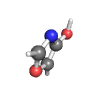
\includegraphics[width= \psize]{satistical_learning/images/m2}}; }] (m2) at (2,2.0){};}
{\node[circle,draw, thick, minimum width = \cssize,path picture={\node at (path picture bounding box.center){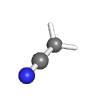
\includegraphics[width= \psize]{satistical_learning/images/m3}}; }] (m3) at (3,1.25){};}
{\node[circle,draw, thick, minimum width = \cssize,path picture={\node at (path picture bounding box.center){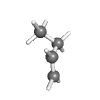
\includegraphics[width= \psize]{satistical_learning/images/m4}}; }] (m4) at (4,0.5){};}
{\node[circle,draw, thick, minimum width = \cssize,path picture={\node at (path picture bounding box.center){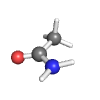
\includegraphics[width= \psize]{satistical_learning/images/m5}}; }] (m5) at (5,-0.25){};}
{\node[circle,draw, thick, minimum width = \cssize,path picture={\node at (path picture bounding box.center){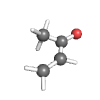
\includegraphics[width= \psize]{satistical_learning/images/m6}}; }] (m6) at (6,-1.0){};}
{\node[circle,draw, thick, minimum width = \cssize,path picture={\node at (path picture bounding box.center){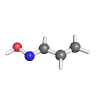
\includegraphics[width= \psize]{satistical_learning/images/m7}}; }] (m7) at (7,-1.75){};}
{\node[circle,draw, thick, minimum width = \cssize,path picture={\node at (path picture bounding box.center){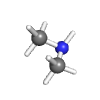
\includegraphics[width= \psize]{satistical_learning/images/m8}}; }] (m8) at (8,-2.5){};}
}


%% mol to vect mapping
\only<2>{
\foreach  \namey / \y in {m1/1.75,m2/1.25,m3/0.75,m4/0.25,m5/-0.25,m6/-0.75,m7/-1.25,m8/-1.75}{
	\visible<1->{\draw [black,thick,->] (\namey) -- (-1,\y) ;}}
\node[anchor=north west] (thislab) at (-1,-2.75) {convert to vectors, preprocess, scale -- not simlpe!};
}

%% rectangles
\visible<2>{\rectDivred{1}{8}{(-1.5,-2)}{(-1.0,2)}{};}
\visible<3>{\rectDivred{1}{8}{(-1.5,-2)}{(-1.0,2)}{0/0,0/1};}
\only<3>{
\node[rotate=90] (thislab) at (-1.75,0.5) {trainning data};
\node[rotate=90, red] (thislab) at (-1.75,-1.5) {test data};
}
\visible<4->{\rectDivred{1}{6}{(-1.5,0)}{(-1.0,3)}{};}
\visible<4->{\rectDivred{1}{2}{(-1.5,-3)}{(-1.0,-2)}{0/0,0/1};}
%% labels to blocks
\only<4>{
	\node[rotate=90] (thislab) at (-1.75,1.5) {trainning data};
	\node[rotate=90, red] (thislab) at (-1.75,-2.5) {test data};
}

%% train phase
\only<1-10>{
%% start learning proc with training data
\visible<5->{
	\node [tbox,minimum width=2.0 cm, text width = 2.0 cm] (traindata) at (\xfarleft,\ytop) {training data};
\node [] (traindatay) at (\xright,\ytop) {};
}
\only<5->{
	\path[draw,dashed] (-1,3) -- (traindata.north west);
	\path[draw,dashed] (-1,0) -- (traindata.south west);	
}

%% show model
\visible<6->{
	\node [tbox,minimum width=2.0 cm, text width = 2.0 cm] (model) at (\xleft,\ymid) {model};
	\draw [thick, black,->] (traindata.south) |-  (model.west);
	\node[anchor=west] (inputslab) at (\xfarleft + \xlabeloffset,0.5*\ymid + 0.5*\ytop)  {inputs, $X$};
}
\only<6-8>{
	\node[anchor=east] (paramslabtemp) at (\xleft - \xlabeloffset,0.5*\ymid + 0.5*\ybot)  {parameters, $W$};
	\draw [thick, black,->] ([yshift=-2cm]model.south) -- (model.south);
}
%% loss needs to be defined out of sequence for reference purposes
\visible<8->{
	\node [tbox,minimum width=2.0 cm, text width = 2.0 cm] (lossf) at (\xright,\ymid) {loss function};
	\draw [thick, black,->] (traindata.east) -- (traindatay.center) -- (lossf.north);
	\node[anchor=east] (labslab) at (\xright - \xlabeloffset,0.5*\ymid + 0.5*\ytop)  {labels, $y(X)$};
}
%% show parameter depedences , out of order to allow modelparams
\visible<9->{
	\node [tbox,minimum width=2.0 cm, text width = 2.0 cm] (modelparams) at (\xmid,\ybot) {update parameters};
	\node[anchor=east] (paramslab) at (\xleft - \xlabeloffset,0.5*\ymid + 0.5*\ybot)  {parameters, $W$};
	\draw [thick, black,->] (modelparams.west) -| (model.south);
	\node[anchor=east] (errorslab) at (\xright - \xlabeloffset,0.5*\ymid + 0.5*\ybot)  {loss, $\mathcal{L}$};
	\draw [thick, black,->] (lossf.south) |- (modelparams.east);
}

\only<8>{
\node[anchor=east] (errorslabtemp) at (\xright - \xlabeloffset,0.5*\ymid + 0.5*\ybot)  {loss, $\mathcal{L}$};
\draw [thick, black,->] (lossf.south) -- ([yshift=-2.cm]lossf.south);
}

%% show predictions
\visible<7->{
\node[anchor=south] (predslab) at (\xmid,\ymid + \ylabeloffset)  {predictions, $\hat{y}(X)$};
\draw [thick, black,->] (model.east) to node [midway,above,label={[label distance=0.15cm]90:}] {} (lossf.west);
}

%% repeat until converged label
\visible<10->{
\node[text width = 2.0cm,text badly centered] (text) at (\xmid,-0.75) {repeat until converged};
\circledarrow{thick, black}{text}{1cm};
}

}

%% testing phase

\only<11->{
%% start learning proc with training data
\node [tbox,minimum width=2.0 cm, text width = 2.0 cm,opacity=0.10] (traindata) at (\xfarleft,\ytop) {training data};
\node [] (traindatay) at (\xright,\ytop) {};
\path[draw,dashed,opacity=0.10] (-1,3) -- (traindata.north west);
\path[draw,dashed,opacity=0.10] (-1,0) -- (traindata.south west);	
\node [tbox,minimum width=2.0 cm, text width = 2.0 cm] (model) at (\xleft,\ymid) {model};
\draw [thick, black,->,opacity=0.10] (traindata.south) |-  (model.west);
\node[anchor=west,opacity=0.10] (inputslab) at (\xfarleft + \xlabeloffset,0.5*\ymid + 0.5*\ytop)  {inputs, $X$};


\node[anchor=west,blue] (paramslabtemp) at (\xleft + \xlabeloffset,0.5*\ymid + 0.5*\ybot)  {parameters, $W$};
\draw [thick, blue,->] ([yshift=-2cm]model.south) -- (model.south);

\node [tbox,minimum width=2.0 cm, text width = 2.0 cm,opacity=0.10] (lossf) at (\xright,\ymid) {loss function};
\draw [thick, black,->,opacity=0.10] (traindata.east) -- (traindatay.center) -- (lossf.north);
\node[anchor=east,opacity=0.10] (labslab) at (\xright - \xlabeloffset,0.5*\ymid + 0.5*\ytop)  {labels, $y(X)$};


\node [tbox,minimum width=2.0 cm, text width = 2.0 cm,opacity=0.10] (modelparams) at (\xmid,\ybot) {update parameters};

\draw [thick, black,->,opacity=0.10] (modelparams.west) -| (model.south);
\node[anchor=east,opacity=0.10] (errorslab) at (\xright - \xlabeloffset,0.5*\ymid + 0.5*\ybot)  {loss, $\mathcal{L}$};
\draw [thick, black,->,opacity=0.10] (lossf.south) |- (modelparams.east);
\node[anchor=east,opacity=0.10] (errorslabtemp) at (\xright - \xlabeloffset,0.5*\ymid + 0.5*\ybot)  {loss, $\mathcal{L}$};
\draw [thick, black,->,opacity=0.10] (lossf.south) -- ([yshift=-2.cm]lossf.south);

\node[anchor=south,opacity=0.10] (predslab) at (\xmid,\ymid + \ylabeloffset)  {predictions, $\hat{y}(X)$};
\draw [thick, black,->,opacity=0.10] (model.east) to node [midway,above,label={[label distance=0.15cm]90:}] {} (lossf.west);


}


\visible<12->{
\node [tbox,minimum width=2.0 cm, text width = 2.0 cm] (testdata) at (\xfarleft,\yphasetwo) {test data};}
\only<12->{
	\path[draw,dashed,red] (-1,-2) -- (testdata.north west);
	\path[draw,dashed,red] (-1,-3) -- (testdata.south west);	
}

\visible<13->{
\draw [thick, black,->] (testdata.north) |-  (model.west);
\node[anchor=east] (testxlab) at (\xfarleft-\xlabeloffset,0.5*\yphasetwo + 0.5*\ymid)  {inputs, $X^*$};
\node[anchor=north] (testpredslab) at (\xmid,\ymid - \ylabeloffset)  {predictions, $\hat{y}(X^*)$};
}
\only<13>{
\draw [thick, black,->] (model.east) --  ([xshift=2cm]model.east) ;
}

\visible<14->{
\node [tbox,minimum width=2.0 cm, text width = 2.0 cm] (evalf) at (\xright,\yphasetwo) {evaluation};
\draw [thick, black,->] (model.east) -|  (evalf.north);

}

\end{tikzpicture}
\end{center}
\end{frame}
%\begin{frame}[t]{Ingredients of supervised learning}
%The basic ingredients are
\begin{enumerate}
	\item Training data $X$ and $y$ -- we write each observation as a row so $X \in \mathbb{R}^{n\times d}$ and $y\in \mathbb{R}^{n}$
	\item A family of possible models $f(\cdot,X)\in \mathcal{T}$, defined by parameters $W$. For example linear: functions \[
	f(X,w)=Xw\]
	\item a loss function -- we'll only use $l_{2}$:
	\[
	\mathcal{L}(y,\hat{y}(x)) = \left\Vert y - \hat{y}(x)\right\Vert_2^2 = \left\Vert y - f(x,W)\right\Vert_2^2 = \left(y - f(x,W)\right)^2
	\]
	\item A way to change $W$ to make $\mathcal{L}$ smaller -- optimization method.
\end{enumerate}
\pause{Note the notation used here.}
%\end{frame}
\subsection{Statistical learning theory}
\begin{frame}[t]{Risk and generalization - I}
Our training data defines the \textit{empirical risk}
\begin{align*}
    \mathcal{E}_{emp}(f) &=\frac{1}{n}\sum_{i=1}^{n}\mathcal{L}(y_i,f(x_i))=\frac{1}{n}\sum_{i=1}^{n}\left(y_i - f(x_i)\right)^2
\end{align*}
we choose the model to minimize $\mathcal{E}_{emp}(f)$ over all the models in $\mathcal{T}$
\begin{align*}
    \hat{f} = \arg\min_{f\in\mathcal{T}} \mathcal{E}_{emp}(f)
\end{align*}
\pause{}
 we actually care about is the overall risk:
\begin{align*}
    \mathcal{E}(f)&=\int\mathcal{L}(y,f(x))p(x,y)dxdy = \mathbb{E}\left[\mathcal{L}(Y,f(X))\right]
\end{align*}
\pause{}
with minimum
\begin{align*}
    f^{*}&= \mathbb{E}\left[\mathcal{L}\left(Y,f(X)\right)\vert X=x\right]
\end{align*}

\end{frame}
\begin{frame}[t]{Risk and generalization - II}
We cannot expect that $f^*$ is in $\mathcal{T}$. The best we can do is $f^{\dagger}$:
\begin{align*}
    f^{\dagger}&= \arg \min_{f\in \mathcal{T}}\mathcal{E}(f) \:& \textrm{(the best model we could pick)}\\
   \uncover<2->{  \hat{f} &= \arg\min_{f\in\mathcal{T}} \mathcal{E}_{emp}(f)\: &\textrm{(the model we do pick)}\\}
      \uncover<2->{      f^{*}&= \mathbb{E}\left[\mathcal{L}\left(Y,f(X)\right)\vert X=x\right]\: &\textrm{(the `truth')}\\}
\end{align*}
\uncover<3->{
We want to generalize,  we want the \textit{excess risk} to be small:
\begin{align*}
 \mathcal{E}(\hat{f}) -      \mathcal{E}(f^{*}) &=    \only<4->{\color{blue}}\left[\mathcal{E}(\hat{f})-\mathcal{E}(f^{\dagger})\right] \only<3- >{\color{black}}  +\only<4->{\color{red}}\left[\mathcal{E}(f^{\dagger})-\mathcal{E}(f^{*})\right]\only<3->{\color{black}} 
\end{align*}}
\uncover<3->{these terms are {\color{blue}\textbf{estimation error}} and {\color{red}\textbf{approximation error}}.}

\end{frame}
\begin{frame}[t]{Risk and generalization - III}
Two critical ideas that are worth noting. Under mild assumptions one can show that:
\begin{enumerate}
\uncover<2->{\item with enough data, the model will generalize. A sufficiently complicated search space $\mathcal{T}$ will cause near-zero approximation error  and we will generalize arbitrarily well. }
\uncover<3->{\item the rate of generalization as we add more data is inversely related to size of the set $\mathcal{T}$, i.e. more complicated spaces of models require more data to generalize. }
\end{enumerate}
\vspace{1cm}
\only<4>{We want $\mathcal{T}$ model to be large/complicated enough to have low approximation error,  \textbf{but no more complicated}.}
\only<5>{ With limited data, we are often better off searching for our model in a simpler family models of that `learn' more robustly and quickly as opposed to very complicated models with lots of parameters.}
\only<6> {Conversely,  a simple model will stop improving with more data past a certain point -- where the approximation error dominates.}
\end{frame}
\begin{frame}[t]{Risk and generalization - IV}
\begin{center}
\begin{tikzpicture}[x=1cm,y=1cm]
%\pgfresetboundingbox
\draw[use as bounding box, anchor = north west,draw=none] (-5.5,-3.25) rectangle (5.5,3.25);
\clip (-5.5,-3.25) rectangle (5.5,3.25);
\node[anchor =north west] (text) at (-5.25,3.25){\begin{minipage}{5.0cm}
\visible<1-8>{Let us use \textbf{polynomials} to estimate:}
\begin{align*}
    y(x) &=\sin(2\pi x)
\end{align*}
Note that $f^{*} \notin \mathcal{T}$!\\
\only<2>{Assume $8$ measurements with noise $\mathcal{N}(0,0.2)$}\\
\only<3-4>{Start with degree $2$...\only<4>{What happens when we increase the order?}}
\only<6-8>{\\ What do the risk terms look like?}
\only<8->{\vspace{1.75cm}\\\color{red}{What happens if we add more data?}}
\end{minipage}};
\visible<1>{\node (figure) at (2.75,0){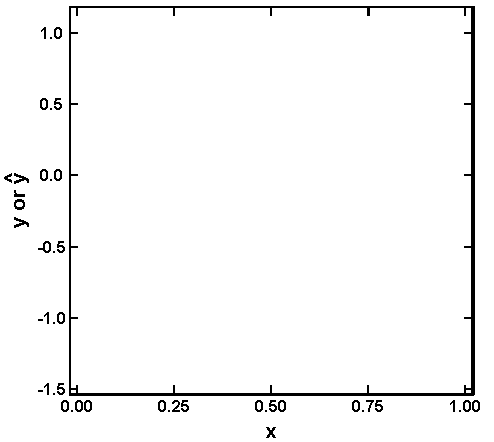
\includegraphics[width=5cm]{satistical_learning/figures/comp_1.pdf}};}
\visible<2>{\node (figure) at (2.75,0){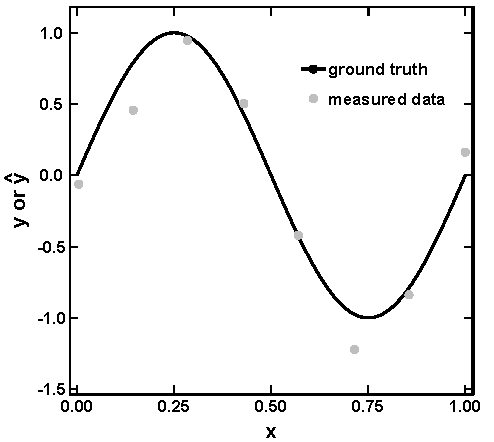
\includegraphics[width=5cm]{satistical_learning/figures/comp_2.pdf}};}
\visible<3>{\node (figure) at (2.75,0){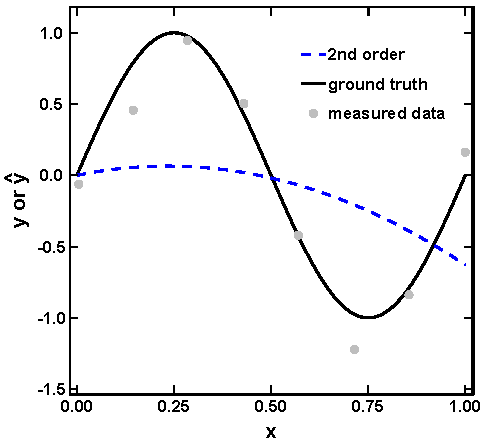
\includegraphics[width=5cm]{satistical_learning/figures/comp_3.pdf}};}
\visible<4>{\node (figure) at (2.75,0){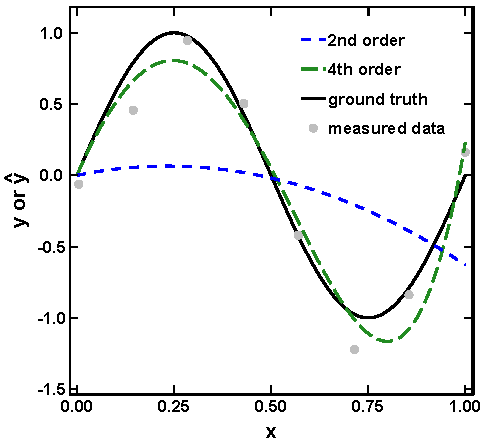
\includegraphics[width=5cm]{satistical_learning/figures/comp_4.pdf}};}
\visible<5-6>{\node (figure) at (2.75,0){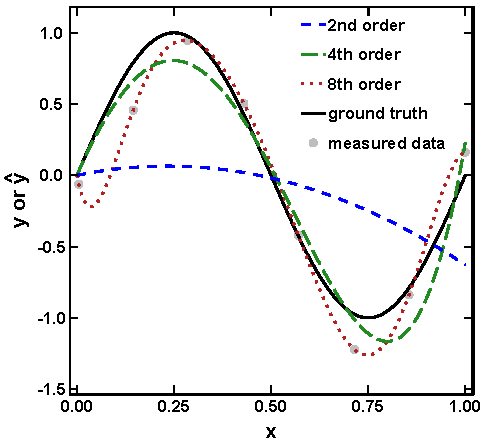
\includegraphics[width=5cm]{satistical_learning/figures/comp_5.pdf}};}
\visible<7->{\node (figure) at (2.75,0){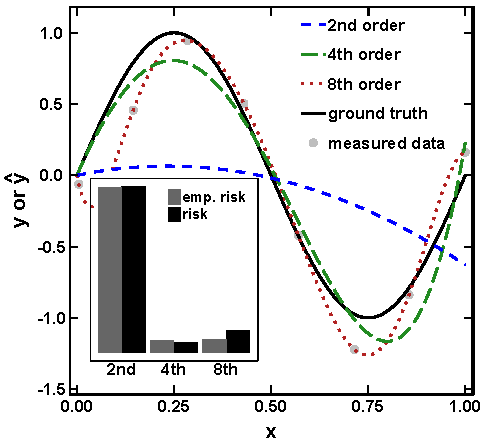
\includegraphics[width=5cm]{satistical_learning/figures/comp_6.pdf}};}
\visible<9->{\node (figure) at (-2.75,0){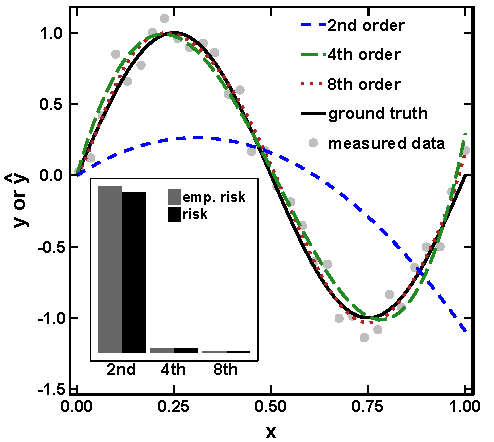
\includegraphics[width=5cm]{satistical_learning/figures/comp_lots_6.pdf}};}
\end{tikzpicture}
\end{center}
\end{frame}
\subsection{Regularization}
\begin{frame}[t]{Controlling Complexity}
\begin{center}
\begin{tikzpicture}[x=1cm,y=1cm]
%\pgfresetboundingbox
\draw[use as bounding box, anchor = north west,draw,dashed,gray] (-5.5,-3.25) rectangle (5.5,3.25);
\clip (-5.5,-3.25) rectangle (5.5,3.25);
\only<6->{\node[anchor =north west] (text) at (-5.25,3.25){\begin{minipage}{10.0cm}Let's return to our previous example:
		\end{minipage}};}
\only<1-5>{\node[anchor =north west] (text) at (-5.25,3.25){\begin{minipage}{10.0cm}
Adapting model complexity to fit the problem is necessary. However, it is not obvious how to do this is a constrolled way.\\
Hence, we need a way prevent over-fitting that is applicable to many different types of model -- \textbf{Regularization}.\\
\visible<2->{We instead choose to minimize:
\begin{small}
\begin{align*}
\mathcal{L}'(y,f(x,w)) &=\mathcal{L}(y,f(x,W)) + \lambda R(W) \\
 \visible<3->{(\textrm{Tiknohov/Ridge})&=\frac{1}{n}\left\Vert y - f(x,W)\right\Vert_2^2 +{\only<4->{\color{red}} \lambda \left\Vert W \right\Vert_2^{2}}}
\end{align*}
\end{small}}
\visible<4->{We choose to {\color{red}penalize terms with large weights}, i.e. complicated functions}.
\visible<5>{\begin{itemize}
\item This makes empirical errors worse.
\item This \textit{can} improve generalization/excess risk.
\end{itemize}}
\end{minipage}};}
\visible<6->{\node (figure) at (-2.75,0){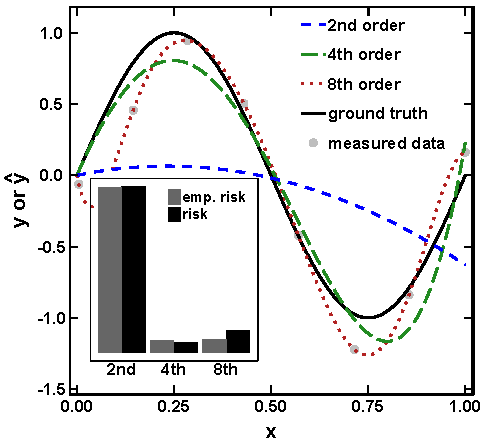
\includegraphics[width=5cm]{satistical_learning/figures/comp_6.pdf}};}
\visible<7->{\node (figure) at (2.75,0){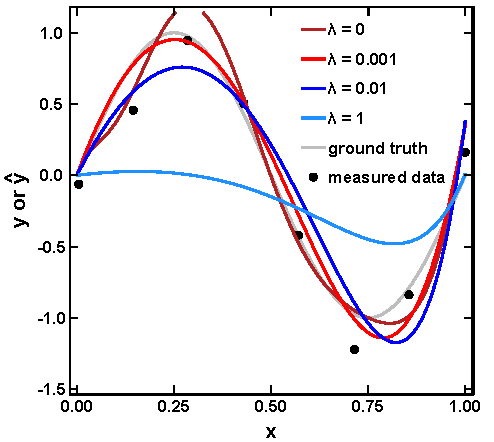
\includegraphics[width=5cm]{satistical_learning/figures/lam_2.pdf}};}
\visible<8->{\node (figure) at (2.75,0){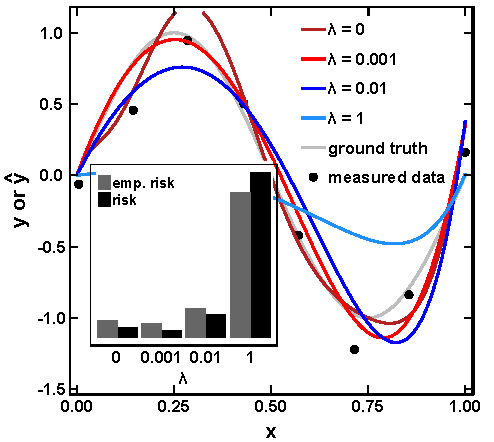
\includegraphics[width=5cm]{satistical_learning/figures/lam_3.pdf}};}
\only<6->{\node[anchor =north west] (text) at (-5.25,-2.75){\begin{minipage}{10.0cm}Remember: larger $\lambda=$ simpler, flatter model. \end{minipage}};}
\end{tikzpicture}
\end{center}
\end{frame}
%
\subsection{Model selection}
\begin{frame}[t]{Controlling Complexity}
\begin{center}
\begin{tikzpicture}[x=1cm,y=1cm]
%\pgfresetboundingbox
\draw[use as bounding box, anchor = north west,draw=none] (-5.5,-3.25) rectangle (5.5,3.25);
\clip (-5.5,-3.25) rectangle (5.5,3.25);
%\node[anchor =north west] (text) at (-5.25,3.25){\begin{minipage}{10.0cm}
%\visible<1->{ We have built up the following picture:
%}
%\end{minipage}};
\visible<1->{\node (figure) at (0,0.75){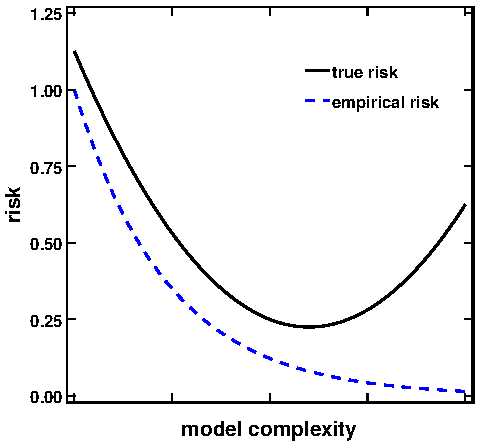
\includegraphics[width=5.25cm]{satistical_learning/figures/scheme_risk}};}
\visible<2->{\node[anchor =north west] (text) at (-5.25,-1.75){\begin{minipage}{10.0cm}
None of this helps us understand a how complicated our model should be.
\visible<3->{Unfortunately, \textbf{errors on our training data cannot tell us the answer}}
\end{minipage}};}
\end{tikzpicture}
\end{center}
\end{frame}
%
\begin{frame}[t]{(Cross)-validation}
\begin{center}
\tikzset{>=latex}
\tikzstyle{block} = [rectangle, draw, fill=blue!20,
text width=1.5cm, text centered, rounded corners, minimum height=1.0cm]	
\def\rectDiv#1#2#3#4#5{%#columns, #rows, rectangle start, rectangle end, list of elements to fill
\draw #3 rectangle #4;
\path #3;
\pgfgetlastxy{\firstx}{\firsty}
\path #4;
\pgfgetlastxy{\secondx}{\secondy}
\pgfmathsetlengthmacro{\xdiff}{\secondx-\firstx}
\pgfmathsetlengthmacro{\ydiff}{\secondy-\firsty}
\pgfmathsetlengthmacro{\myxstep}{\xdiff/#1}
\pgfmathsetlengthmacro{\myystep}{\ydiff/#2}
\foreach \x in {1,...,#1}{
	\draw ($#3 +\x*(\myxstep,0)$) -- ($#3 +(0,\ydiff) +\x*(\myxstep,0)$);
}
\foreach \y in {1,...,#2}{
	\draw ($#3 +\y*(0,\myystep)$) -- ($#3 +(\xdiff,0) +\y*(0,\myystep)$);
}
\foreach \i/\j in {#5}{
	\path[fill=darkgreen!20,draw] ($#3 + (\i*\myxstep,\j*\myystep)$) rectangle ($#3 + (\i*\myxstep,\j*\myystep) + (\myxstep,\myystep)$);
}
}
\def\rectDivred#1#2#3#4#5{%#columns, #rows, rectangle start, rectangle end, list of elements to fill
\draw #3 rectangle #4;
\path #3;
\pgfgetlastxy{\firstx}{\firsty}
\path #4;
\pgfgetlastxy{\secondx}{\secondy}
\pgfmathsetlengthmacro{\xdiff}{\secondx-\firstx}
\pgfmathsetlengthmacro{\ydiff}{\secondy-\firsty}
\pgfmathsetlengthmacro{\myxstep}{\xdiff/#1}
\pgfmathsetlengthmacro{\myystep}{\ydiff/#2}
\foreach \x in {1,...,#1}{
	\draw ($#3 +\x*(\myxstep,0)$) -- ($#3 +(0,\ydiff) +\x*(\myxstep,0)$);
}
\foreach \y in {1,...,#2}{
	\draw ($#3 +\y*(0,\myystep)$) -- ($#3 +(\xdiff,0) +\y*(0,\myystep)$);
}
\foreach \i/\j in {#5}{
	\path[fill=red!20,draw] ($#3 + (\i*\myxstep,\j*\myystep)$) rectangle ($#3 + (\i*\myxstep,\j*\myystep) + (\myxstep,\myystep)$);
}
}

\begin{tikzpicture}[x=1cm,y=1cm]
%\pgfresetboundingbox
\draw[use as bounding box, anchor = north west,draw,dashed,gray] (-2,-3.25) rectangle (9,3.25);
\clip (-2,-3.25) rectangle (9.0,3.25);
\node (ds) at (0,0){};
\node (dsy) at (0,4){};
\node (dsx) at (4,0){};

\visible<1->{\rectDivred{1}{6}{(-1.5,0)}{(-1.0,3)}{};}
\visible<1->{\rectDivred{1}{2}{(-1.5,-3)}{(-1.0,-2)}{0/0,0/1};}
%% labels to blocks
\only<1->{
\node[rotate=90] (thislab) at (-1.75,1.5) {trainning data};
\node[rotate=90, red] (thislab) at (-1.75,-2.5) {test data};
}


\visible<2>{\rectDiv{1}{6}{(0,-1)}{(0.5,2)}{};}
\visible<3-8>{\rectDiv{1}{6}{(0,-1)}{(0.5,2)}{0/0};}
\visible<3>{\draw [decorate,decoration={brace,amplitude=10pt,raise=4pt},yshift=0pt]
	(0,-1) -- (0,2) node [black,midway,xshift=-1.25cm,rotate=90] {\footnotesize $\text{k-folds}$};}
\visible<2-11>{\draw[black,dashed] (-1,0)--(0,-1);}
\visible<2-11>{\draw[black,dashed] (-1,3)--(0,2);}


\visible<4-8>{\rectDiv{1}{6}{(1,-0.5)}{(1.5,2)}{};}
\visible<4-8>{\rectDiv{1}{1}{(1,-1.5)}{(1.5,-1.0)}{0/0};}
\visible<4-8>{\node[darkgreen,anchor=north] (thislab) at (0.5,-1.75) {validation data};}

\visible<4-8>{\draw[black,dashed] (0.5,-1)--(1.0,-1.5);}
\visible<4-8>{\draw[black,dashed] (0.5,-0.5)--(1.0,-1.0);}

\visible<5-8>{\node[block] (trained) at (3.5,0.75){model A};}
\visible<5>{\node (LAlab) at (3.5,2.25){\Large $\lambda _A$};}
\visible<5>{\draw[black,very thick,->] (LAlab) -- (trained);}
\foreach \x in {1.5}
\foreach \y in {-0.25,0.25,0.75,1.25,1.75}{
	\visible<5-8>{\draw [black] (\x,\y) -- (trained.west);}}

\visible<6-8>{\draw[red,very thick,->] (1.5,-1.25) -| node[right] {predict} ([xshift=0,yshift=-1.0cm]trained.south) --(trained.south);}


\visible<8>{\rectDivred{1}{6}{(6,-1)}{(6.5,2)}{0/0};}
\visible<8>{\draw[red,very thick,->] (trained.east) -- (6.0,-0.75);}
\visible<8>{\node[red,anchor = west] at (6.75, -0.75){error}  ;}

\visible<8-11>{\node[anchor = west] at (3.5, -1.75){repeat for all $k$ folds};}

\visible<9>{\rectDiv{1}{6}{(0,-1)}{(0.5,2)}{0/1};}
\visible<9>{\rectDivred{1}{6}{(6,-1)}{(6.5,2)}{0/1,0/0};}
\visible<9>{\node[red,anchor = west] at (6.75, -0.25){error};}
\visible<9>{\draw[red,very thick,->] (0.5,-0.25) -- (6.0,-0.25);}
\visible<10>{\rectDiv{1}{6}{(0,-1)}{(0.5,2)}{0/2};}
\visible<10>{\draw[red,very thick,->] (0.5,0.25) -- (6.0,0.25);}
\visible<10>{\node[red,anchor = west] at (6.75, 0.25){error};}
\visible<10>{\rectDivred{1}{6}{(6,-1)}{(6.5,2)}{0/2,0/1,0/0};}
%% all done 
\visible<11-12>{\rectDivred{1}{6}{(6,-1)}{(6.5,2)}{0/2,0/1,0/0,0/3,0/4,0/5,0/6};}
\visible<11>{\rectDiv{1}{6}{(0,-1)}{(0.5,2)}{};}
\visible<12>{\draw [decorate,decoration={brace,amplitude=10pt,raise=4pt},yshift=0pt]
	(6,-1) -- (6,2) node [text badly centered,midway,xshift=-2.0cm, text width = 2 cm] { $\text{average  error}=\color{red}\textrm{CV error}$};}

\visible<13-15>{\node[anchor = west] at (-0.75, -3.0){\textbf{CV error way is a fair way to compare models}};}

\visible<13-15>{\node[block] (MA) at (1,2){model A};}
\visible<13-15>{\node[red, anchor= west] (CVA) at (3.0,2.0){CV error A};}
\visible<13-15>{\path[draw,red,very thick,->] (-1.0,1.5) -- (MA.west);}
\visible<13-15>{\path[draw,red,very thick,->] (MA.east) -- (CVA);}

\visible<14-15>{\node[block] (MB) at (1,0){model B};}
\visible<14-15>{\node[red, anchor= west] (CVB) at (3.0,0.0){CV error B};}
\visible<14-15>{\path[draw,red,very thick,->] (-1.0,1.5) -- (MB.west);}
\visible<14-15>{\path[draw,red,very thick,->] (MB.east) -- (CVB);} 
 
\visible<15>{\node[block] (MC) at (1,-2){model C};}
\visible<15>{\node[red, anchor= west] (CVC) at (3.0,-2.0){CV error C};}
\visible<15>{\path[draw,red,very thick,->] (-1.0,1.5) -- (MC.west);} 
\visible<15>{\path[draw,red,very thick,->] (MC.east) -- (CVC);}


\visible<16>{\node[block] (BM) at (1,0){model B};}
\visible<16>{\node[red, anchor= west] (BP) at (3.0,0){predictions};}
\visible<16>{\path[draw,red,very thick,->] (-1.0,-2.5) -| (BM.south);}
\visible<16>{\path[draw,red,very thick,->] (BM.east) -- (BP);}
%
%\visible<1>{\node [circle,draw=red,fill=red,opacity=0.25] () at (6,3.25) {\huge 1};}
%\visible<2>{\node [circle,draw=red,fill=red,opacity=0.25] () at (6,3.25) {\huge 2};}
%\visible<3>{\node [circle,draw=red,fill=red,opacity=0.25] () at (6,3.25) {\huge 3};}
%\visible<5-7>{\node [circle,draw=red,fill=red,opacity=0.25] () at (6,3.25) {\huge 4};}
%\visible<8>{\node [circle,draw=red,fill=red,opacity=0.25] () at (6,3.25) {\huge 5};}



%\visible<1-4>{\rectDiv{1}{12}{(-1.5,-2.0)}{(-0.5,3.0)}{0/0};}
%\visible<1-4>{\rectDiv{1}{10}{(0,-2.5)}{(1,2.5)}{0/0};}
%\visible<2-4>{\rectDiv{1}{9}{(3,-1.5)}{(4,3)}{};}
%\visible<2-4>{\rectDiv{1}{1}{(3,-3)}{(4,-2.5)}{0/0};}


%%#columns, #rows, rectangle start, rectangle end, list of elements to fill

%
%\visible<4->{\rectDivred{1}{10}{(8,-2.5)}{(9,2.5)}{0/0};}

%
%\visible<5-7>{\draw[red,very thick,->,bend left] (1,2.25) to node[label={[label distance=1.0cm]-90:{repeat for all folds}}]{} (trained.west);}
%\visible<5-7>{\draw[red,very thick,->,bend right] (trained.east) to node[below] {} (8,0) ;}
%%\visible<6>{\rectDiv{1}{10}{(0,-2.5)}{(1,2.5)}{0/1,0/2,0/3,0/4,0/5,0/6,0/7,0/8,0/9};}
%\visible<5>{\rectDiv{1}{10}{(0,-2.5)}{(1,2.5)}{0/1};}
%\visible<5->{\rectDivred{1}{10}{(8,-2.5)}{(9,2.5)}{0/1};}
%\visible<6>{\rectDiv{1}{10}{(0,-2.5)}{(1,2.5)}{0/2};}
%\visible<6->{\rectDivred{1}{10}{(8,-2.5)}{(9,2.5)}{0/2};}
%\visible<7>{\rectDiv{1}{10}{(0,-2.5)}{(1,2.5)}{0/3};}
%\visible<7->{\rectDivred{1}{10}{(8,-2.5)}{(9,2.5)}{0/3};}
%\visible<8>{\rectDiv{1}{10}{(0,-2.5)}{(1,2.5)}{0/9};}
%\visible<8->{\rectDivred{1}{10}{(8,-2.5)}{(9,2.5)}{0/0,0/1,0/2,0/3,0/4,0/5,0/6,0/7,0/8,0/9};}

\end{tikzpicture}
\end{center}
\end{frame}
\subsection{Conclusion}
\begin{frame}[t]{Conclusion}
In summary:
\vspace{1cm}
\pause{}
\begin{enumerate}
	\item We train models by changing their parameters to reduce errors on training data \pause{}
	\item More complicated models learn more slowly, but have more capacity\pause{}
	\item Regularization helps control complexity\pause{}
	\item Cross-validation (and related techniques)  must be used to choose hyperparameters\pause{}
\end{enumerate}
\vspace{1cm}
Deep neural networks (might) need better theories.
\end{frame}